% A simple LaTeX template for an article
\documentclass[12pt]{article}

\usepackage{tikz}
\usepackage{xcolor}

% Define colors
\definecolor{phase1}{HTML}{3182CE}  % Blue
\definecolor{phase2}{HTML}{38A169}  % Green
\definecolor{phase3}{HTML}{E53E3E}  % Red

% Document information
\title{Gantt Chart}
\author{Jun Cao}
\date{\today}

\begin{document}

\maketitle

\begin{abstract}
Your abstract goes here.
\end{abstract}

\section{Introduction}
This is a minimal example of a LaTeX article with a Gantt chart.

\section{Gantt Chart}
Figure~\ref{fig:gantt} is a Gantt chart for the project.

% Insert the Gantt chart and resize it to the width of the text
\begin{figure}[htbp]
    \centering
    \resizebox{\textwidth}{!}{%
        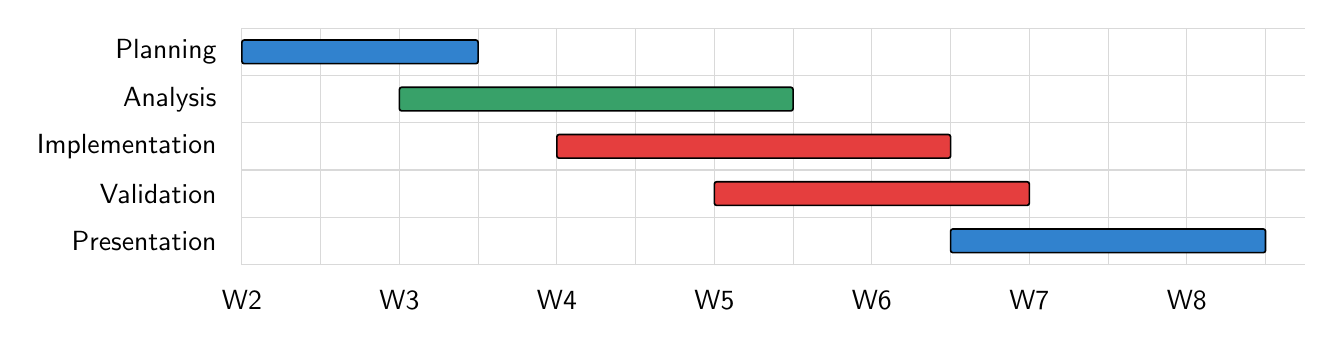
\begin{tikzpicture}[
    every node/.style={font=\sffamily},     % Set font
    bar/.style={                            % Define the style for the bars
        rectangle,                          % Rectangle shape
        rounded corners=0.8pt,              % Rounded corners
        minimum height=8pt,                 % Minimum height of the bar
        line width=0.6pt,                   % Border line width
        draw=black                          % Border line color
    }
]

% Grid range based on the number of weeks or periods, etc.
% (-0.2pt,-0.2pt) instead of (0,0) to ensure the grid corners are not cut off
% xstep can be added to increase the resolution of days
\draw[gray!30] (-0.2pt,-0.2pt) grid[ystep=0.6, xstep=1] (13.5,3);

% Week labels: W2 to W8
\foreach \x in {0,2,...,12} {
    \draw (\x,-0.2) node[below] {W\the\numexpr\x/2+2};
}

% Tasks
\node[anchor=east] at (-0.2,2.7) {Planning};
% Task bar, 
\draw[bar, fill=phase1] (0,2.55) rectangle +(3,0.3);

\node[anchor=east] at (-0.2,2.1) {Analysis}; 
\draw[bar, fill=phase2] (2,1.95) rectangle +(5,0.3);

\node[anchor=east] at (-0.2,1.5) {Implementation};
\draw[bar, fill=phase3] (4,1.35) rectangle +(5,0.3);

\node[anchor=east] at (-0.2,0.9) {Validation};
\draw[bar, fill=phase3] (6,0.75) rectangle +(4,0.3);

\node[anchor=east] at (-0.2,0.3) {Presentation};
\draw[bar, fill=phase1] (9,0.15) rectangle +(4,0.3);

\end{tikzpicture}%
    }
    \caption{Gantt Chart}\label{fig:gantt}
\end{figure}

\end{document}
